\documentclass[hidelinks,12pt]{article}

\usepackage{amsmath}    % need for subequations
\usepackage{graphicx}   % need for figures
\usepackage{verbatim}   % useful for program listings
\usepackage{color}      % use if color is used in text
\usepackage{subfigure}  % use for side-by-side figures
\usepackage{hyperref}   % use for hypertext links, including those to external documents and URLs
\usepackage{units}
\usepackage[numbered]{matlab-prettifier} % including matlab w/ syntax highlighting
\usepackage[T1]{fontenc} % prettier matlab font
\lstMakeShortInline[style=Matlab-editor]| % matlab inline escape character
\graphicspath{ {./Figures/} }

\usepackage[
top    = 2.75cm,
bottom = 2.50cm,
left   = 3.00cm,
right  = 2.50cm]{geometry}



% don't need the following. simply use defaults
\setlength{\baselineskip}{16.0pt}    % 16 pt usual spacing between lines



\begin{document}
\pagenumbering{gobble}
\begin{center}
  {\huge Homework 5}\\
  \vspace{10px}
  
\includegraphics{Logo} \\
  Date of Submission:\\
  February 25, 2019\\
  \vspace{30px}
  \rule{300px}{0.5px} \\
  Thorne Wolfenbarger \\
  \href{mailto:wolfent1@my.erau.edu}{wolfent1@my.erau.edu} \\
  \vspace{30px}
  Submitted to: \\
  Professor Kaela Martin \\
  College of Engineering \\
  \vspace{40px}
  In Partial Fulfillment \\
  of the Requirements of \\
  \vspace{10px}
  AE 313 \\
  Space Mechanics \\
  Spring, 2019 \\
\end{center}

\pagenumbering{roman}
{\tableofcontents\let\clearpage\relax}
\clearpage
\pagenumbering{arabic}
\newpage
\begin{flushleft}
\begin{large}
  Knowns
\end{large}\\
\begin{center}
  \begin{tabular}{ccc}
    a = 42,170 km & e = 0.01053 & $\Omega$ = 14.89$^\circ$\\$\omega$ = 318.4$^\circ$ & $i$ = 14.37$^\circ$ & $\theta_1^*$ = 184.2$^\circ$
  \end{tabular}
\end{center}

\section{Current Position And Velocity}
Find the current position and velocity ($\vec{r}_1,\vec{v}_1$) in ECI and perifocal coordinates.
\begin{center}
  $\vec{r}_1 = (-3.9158 \hat{x} + 1.5532 \hat{y} + 0.6423 \hat{z})\cdot 10^4~km = (-4.2498 \hat{e} -0.3121 \hat{p})\cdot 10^4~km$\\
  $\vec{v}_1 = -1.1820 \hat{x} - 2.7383 \hat{y} - 0.6002 \hat{z}~\nicefrac{km}{s} = 0.2252 \hat{e} - 3.0340 \hat{p}~\nicefrac{km}{s}$
\end{center}
\vspace{5px}
% MATLAB Code
\begin{lstlisting}[frame=lines,style=Matlab-editor,basicstyle = \mlttfamily]
% 1. Find the current position and velocity in ECI and perifocal coordinates
p = a*(1-e^2);
h = sqrt(MU*p);
r1 = p/(1+e*cosd(true_a1));

vr1_rth = [r1 0 0]';
vv1_rth = [h*e/p*sind(true_a1) h/r1 0]';

AOL1 = AOP + true_a1;
rth_eci = rot_rth_eci(RAAN,inc,AOL1);

vr1_eci = rth_eci*vr1_rth;
vv1_eci = rth_eci*vv1_rth;

vr1_peri = r1*[cosd(true_a1) sind(true_a1) 0]';
vv1_peri = [-h/p*sind(true_a1) h/p*(e+cosd(true_a1)) 0]';
\end{lstlisting}
\section{Time To Send The Message}
You need to send the message by the time E = 15$^\circ$. How long do you have until $t_2$?\\
Time until E = $15^\circ$: t = $4.5618\cdot 10^4~sec = 12.6716~hours = 0.528~days$
\vspace{5px}
\begin{lstlisting}[frame=lines,style=Matlab-editor,basicstyle = \mlttfamily]
% 2. You need to send the message by the time E=15deg. How long do you have
% until t2?
period = 2*pi*sqrt(a^3/MU);
E2 = 15; %deg
E2_rad = E2*pi/180;
E1 = 2*atand(tand(true_a1/2)/sqrt((1+e)/(1-e)));
E1_rad = E1*pi/180;

dt = sqrt(a^3/MU)*(E2_rad - E1_rad - (e*sin(E2_rad) - e*sin(E1_rad)));
\end{lstlisting}
\section{New Position And Velocity}
What is the new position and velocity ($\vec{r}_2, \vec{v}_2$) in ECI and perifocal coordinates?\\
\begin{center}
  $\vec{r}_2 = (4.0746 \hat{x} -0.7798 \hat{y} -0.4613 \hat{z})\cdot 10^4~km = (4.0289 \hat{e} + 1.0914 \hat{p})\cdot 10^4~km$\\
  $\vec{v}_2 = 0.6526 \hat{x} + 2.9573 \hat{y} + 0.6892 \hat{z}~\nicefrac{km}{s} = -0.8039 \hat{e} + 3.0000 \hat{p}~\nicefrac{km}{s}$
\end{center}
\begin{lstlisting}[frame=lines,style=Matlab-editor,basicstyle = \mlttfamily]
% 3. What is the new position and velocity in ECI and perifocal coordinates?
r2 = a*(1-e*cos(E2_rad));
true_a2 = 2*atan2d(sqrt((1+e)/(1-e))*tan(E2_rad/2),1);
vr2_rth = [r2 0 0]';
vv2_rth = [h*e/p*sind(true_a2) h/r2 0]';

AOL2 = AOP + true_a2;
rth_eci = rot_rth_eci(RAAN,inc,AOL2);

vr2_eci = rth_eci*vr2_rth;
vv2_eci = rth_eci*vv2_rth;

vr2_peri = r2*[cosd(true_a2) sind(true_a2) 0]';
vv2_peri = [-h/p*sind(true_a2) h/p*(e+cosd(true_a2)) 0]';
\end{lstlisting}
\section{Latitude And Longitude}
Find the latitiude and longitude at the two positions.\\
\begin{center}
  \begin{tabular}{cc}
    $\phi_1 = 8.6698^\circ$ & $\lambda_1 = -49.9545^\circ$\\
    $\phi_2 = -6.3452^\circ$ & $\lambda_2 = -49.7477^\circ$
  \end{tabular}
\end{center}
\begin{lstlisting}[frame=lines,style=Matlab-editor,basicstyle = \mlttfamily]
% 4. Find the latitiude and longitide at the two positions
dt_days = dt/60/60/24;
rot_earth = 7.2921151467*10^-5; %rad
tu1 = juliandate(datetime('2019-03-06 03:00:00')) - 2451545;
tu2 = juliandate(datetime('2019-03-06 03:00:00')) - 2451545;

theta_era1 = 2*pi*(0.7790572732640 + 1.00273781191135448*tu1);
theta_era1 = mod(theta_era1,2*pi)*180/pi;
theta_era2 = 2*pi*(0.7790572732640 + 1.00273781191135448*tu2);
theta_era2 = mod(theta_era2,2*pi)*180/pi;

eci_ecef1 = rot_eci_ecef(theta_era1);
eci_ecef2 = rot_eci_ecef(theta_era2);
vr1_ecef = eci_ecef1*vr1_eci;
vr2_ecef = eci_ecef2*vr2_eci;


alpha1 = atan2d(cosd(inc)*sind(AOL1),cosd(AOL1));
alpha2 = atan2d(cosd(inc)*sind(AOL2),cosd(AOL2));
theta_gr1 = theta_era1+180/pi*rot_earth*0;
theta_gr2 = theta_era2+180/pi*rot_earth*dt;

lat1 = asind(vr1_ecef(3)/r1);
long1 = alpha1 + RAAN - theta_gr1;
lat2 = asind(vr2_ecef(3)/r2);
long2 = alpha2 + RAAN - theta_gr2;
long2 = mod(long2,-360);
\end{lstlisting}
\newpage
\section{Ground Track}
Create a ground track between the two position using MATLAB. Mark the starting location.
\begin{figure}[!htb]
  \center
  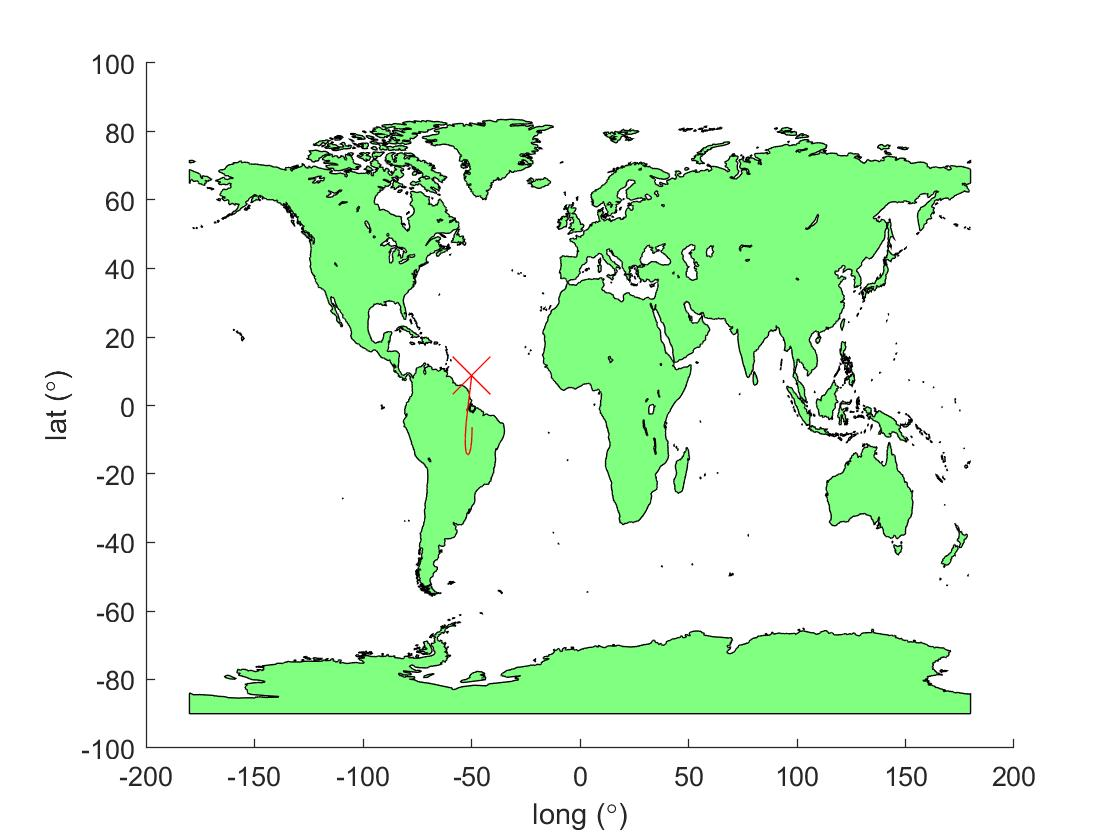
\includegraphics[scale=0.4]{LATLONG}
  \caption{Latitude vs. Longitude}
  \label{}
\end{figure}\\
\begin{lstlisting}[frame=lines,style=Matlab-editor,basicstyle = \mlttfamily]
% 5. Create a ground track between the two positions using MATLAB. Mark the
% starting location.

true_a_array = linspace(true_a1, true_a2+360, 1000);
r_array = p./(1+e*cosd(true_a_array));
% E_array = acosd(-(r_array/a-1)/e).*sign(true_a_array);
E_array = 2*atand(tand(true_a_array/2)/sqrt((1+e)/(1-e)));
E_array_rad = E_array*pi/180;

dt_array = sqrt(a^3/MU)*(E_array_rad - E1_rad - (e*sin(E_array_rad) - e*sin(E1_rad)));

theta_era = theta_era1;
theta_gr_array = theta_era+180/pi*rot_earth*dt_array;


theta_array = AOP + true_a_array;
lat_array = asind(sind(inc)*sind(theta_array));

alpha_array = atan2d(cosd(inc)*sind(theta_array),cosd(theta_array));
long_array = alpha_array + RAAN - theta_gr_array;

figure; hold on;
geoshow("landareas.shp","FaceColor",[0.5 1.0 0.5]);
geoshow(lat_array, long_array,'Color','red');
geoshow(lat_array(1),long_array(1),'DisplayType','Point','Marker','x','Markersize',20);
\end{lstlisting}
\newpage
\section{Can You Send The Message?}
Assume that you have a ground station in Prescott (34.54 N, 112.4685 W, 1.64 km above mean equatorial). Plot the elevation angle versus time passed. If the ground station needs a minimum elevation angle of 10 degrees, how much time is the TDRS visible? Can you send your urgent message to the TDRS?\\
\begin{figure}[!htb]
  \center
  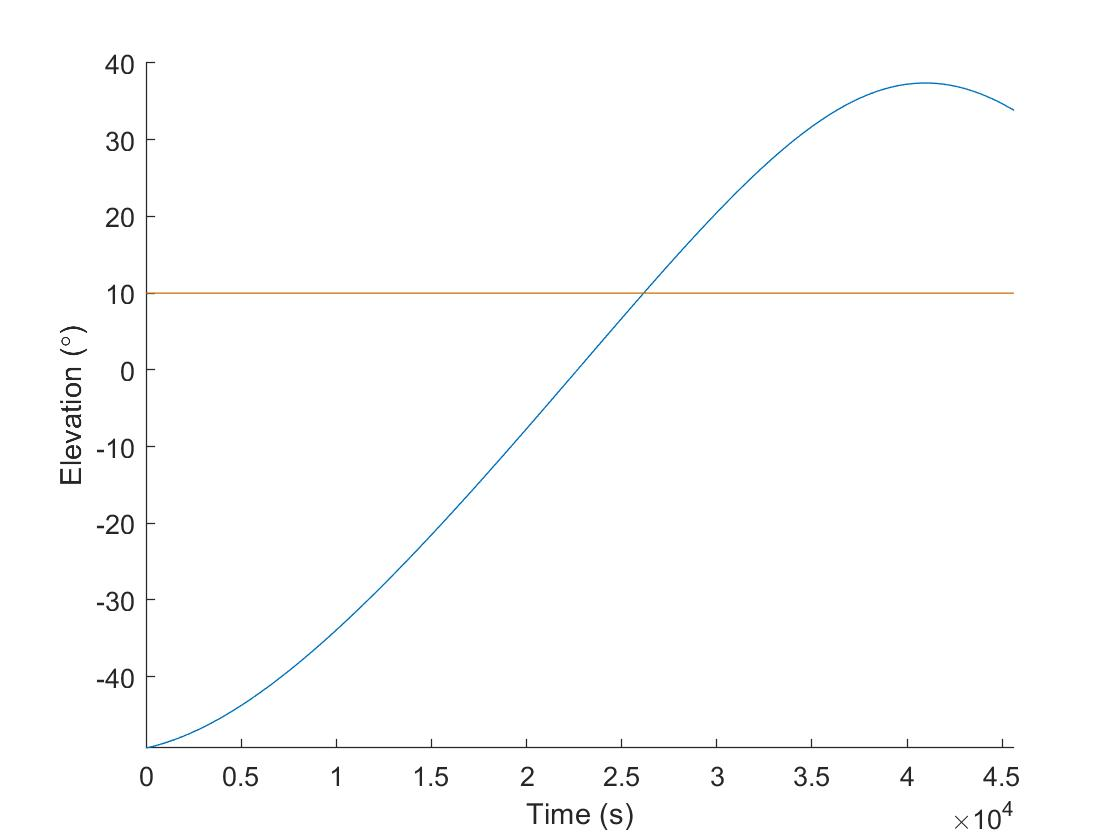
\includegraphics[scale=0.4]{ELEVATIONTIME}
  \caption{Elevation vs. Time}
  \label{}
\end{figure}
In Part 2, "Time To Send The Message", we were informed that we have until E = 15 degrees to send our message. We found that it will take 12.6716 hours to reach our E = 15 degrees limit, beginning on March 6, 2019 at 03:00:00.000. As shown in the above plot, it will take only 7.2751 hours for TDRS to become visible to our ground station. Once visible, the TDRS will remain visible for 5.3965 hours. Therefore, because TDRS becomes and remains visible for well within our allowable range, we will be able to send our urgent message as early as 10:16:30.36.
\vspace{5px}
\begin{lstlisting}[frame=lines,style=Matlab-editor,basicstyle = \mlttfamily]
% 6. Assume you have the ground station in Prescott. Plot the elevation angle
% versus time passed. If the ground station needs a minimum elevation angle
% of 10 degrees, how much time is the TDRS visible? Can you send your
% urgent message to the TDRS?
min_elevation = 10; %deg
radius_e = 6378; %km
lat_gs = 34.54; %deg
long_gs = 112.4685; %deg
h_gs = 1.64; %km
vr_e_gs = [0 0 radius_e+h_gs]'; %km

elevation_array = zeros(1,length(r_array));
for i = 1:length(r_array)
    vr_rth = [r_array(i) 0 0]';
    rth_eci = rot_rth_eci(RAAN, inc, theta_array(i));
    eci_ecef = rot_eci_ecef(theta_era);
    vr_ecef = eci_ecef*rth_eci*vr_rth;

    ecef_sez = rot_ecef_sez(long_gs, lat_gs);
    vr_sez = ecef_sez*vr_ecef;

    vr_e_sc = vr_sez;

    vr_gs_sc = vr_e_sc - vr_e_gs;

    elevation_array(i) = asind(vr_gs_sc(3)/norm(vr_gs_sc));
end

figure(2)
hold on;
plot(dt_array, elevation_array)
line([0 dt_array(end)], [10 10],'Color',[0.78 0.43 0.02])
xlabel('Time (s)')
ylabel('Elevation (\circ)')
q = 1;
while elevation_array(q)<10
    q = q + 1;
end
time_start = dt_array(q);
time_end = dt_array(end);
time_above_minimum = time_end - time_start;
time_above_minimum_hours = time_above_minimum/60/60;
\end{lstlisting}
\newpage
\section{Why?}
Why would the TDRS be in such an orbit?\\
\vspace{5px}
The TDRS is a relay satellite intended to be in a geosynchronous orbit. The purpose of such an orbit is to maximize the amount of time that signals can be transmitted through TDRS from a well positioned ground station.


\end{flushleft}
\newpage
HW5.m
\begin{lstlisting}[frame=lines,style=Matlab-editor,basicstyle = \mlttfamily]
clc; clear all; close all

%constants
MU = 42828;

% Problem 1
vr = [-2089.6 -2515.7 -6382.0];
vv = [2.1744 0.76911 0.13452];

r = norm(vr)
v = norm(vv)

vh = cross(vr, vv);
h = norm(vh);

syms a
energy_eqn = v^2/2 - MU/r == -MU/(2*a)
energy = v^2/2 - MU/r
a = double(solve(energy_eqn, a))

syms e
h_eqn = h == sqrt(MU*a*(1-e^2))
e = double(solve(h_eqn,e))
e = max(e)

syms E
E_eqn = r == a*(1-e*cos(E));
E = double(solve(E_eqn,E));
E = -min(E) %Because it is descending.

syms time_since_p
time_since_p_eqn = sqrt(MU/a^3)*time_since_p == E - e*sin(E);
time_since_p = double(solve(time_since_p_eqn,time_since_p))

% Problem 2
p = h^2/MU;
true_a = -acos(p/(r*e) - 1/e)
vv_rt = [h*e/p*sin(true_a) h/r 0] % answer

% Problem 3
E1 = E;
t1 = time_since_p;
vr1 = vr;
vv1 = vv;
r1 = r;
v1 = v;
t2 = time_since_p + 12*60*60;
n = sqrt(MU/a^3);
M = n*t2;
E2 = fzero(@(x) x-e*sin(x)-M, 0);
f = 1 - a/r*(1-cos(E2-E1));
g = (t2 - t1) - sqrt(a^3/MU)*(E2 - E1 - sin(E2 - E1));

vr2 = f*vr + g*vv;
r2 = norm(vr2);
fdot = -sqrt(MU*a)/(r2*r1)*sin(E2-E1);
gdot = 1 - a/r2*(1-cos(E2-E1));

vv2 = fdot*vr1 + gdot*vv1 % intertial unit vectors

true_a2 = -acos(p/(r2*e) - 1/e)

vv2_rt = [h*e/p*sin(true_a2) h/r2 0] % radial-tangential

% Problem 4
vr2_peri = [r2*cos(true_a2) r2*sin(true_a2) 0]
vv2_peri = sqrt(MU/p)*[-sin(true_a2) e+cos(true_a2) 0]

% Problem 5

% find i theta omega
syms inc
h_hat = cross(vr2, vv2)/norm(cross(vr2, vv2))
inc_eqn = cos(inc) == dot(h_hat, [0 0 1])
inc = double(solve(inc_eqn,inc))
inc = max(inc)

syms RAAN
RAAN_eqn_1 = sin(RAAN)*sin(inc) == dot(h_hat, [1 0 0])
RAAN_eqn_2 = -cos(RAAN)*sin(inc) == dot(h_hat, [0 1 0])
RAAN1 = double(solve(RAAN_eqn_1));
RAAN2 = double(solve(RAAN_eqn_2));
RAAN = min(RAAN1)*180/pi

syms arg_peri
r1_hat = vr1/norm(vr1)
theta_hat = cross(r1_hat, h_hat)/norm(cross(r1_hat, h_hat))
syms theta
theta_eqn_1 = sin(inc) * sin(theta) == dot(r1_hat, [0 0 1])
theta_eqn_2 = sin(inc) * cos(theta) == dot(theta_hat, [0 0 1])
theta1 = double(solve(theta_eqn_1, theta))
theta2 = double(solve(theta_eqn_2, theta))
theta = intersect(theta1, theta2)
arg_peri_eqn = arg_peri == theta - true_a
arg_peri = double(solve(arg_peri_eqn, arg_peri))
\end{lstlisting}

\end{document}
